\subsection{Dalvik Executionable File Format} \label{subsection:android-dex}
As explained in chapter~\cite{subsection:foundation-android-package}, Android applications deliver their code in \gls{dex} bytecode and are executed by the \gls{dvm}.
The dex file format is compiled from Java bytecode.
Java and the \gls{dvm} differ significantly in how they execute code.
While the Java \gls{vm} is stack-based the \gls{dvm} is register-based.
Dalvik bytecode is more suited to run on the ARM architecture since it supports direct mapping from dex registers to the registers of the ARM processor.
Registers in \gls{dex} bytecode are 32bits wide and store values such as integers or float values.
In case there are 64bit values, adjacent registers are used to store it.
The Java bytecode is actually more compact since it uses 8bit instructions while \gls{dex} bytecode has instructions of 16bit multiples.
The \gls{dex} bytecode supports 218 valid opcodes which have a dest-source ordering for its arguments.
\newline
\begin{figure}[h]
    \centering
    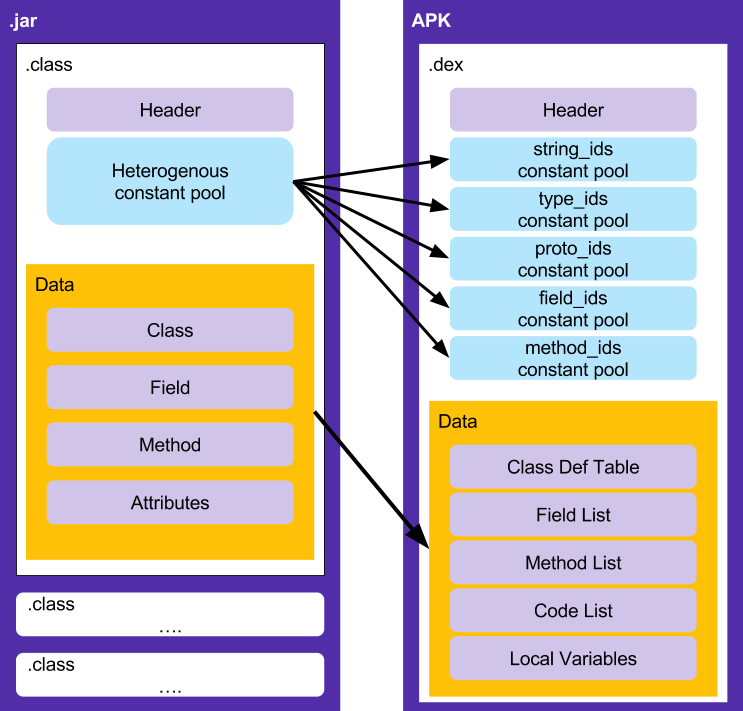
\includegraphics[width=0.5\textwidth]{data/java.png}
    \caption{\gls{jar} to \gls{apk} transformation \cite{googleDalvik}}
    \label{fig:java}
\end{figure}

The arguments for Java instructions are not stored inside the method but as a reference, pointing to the variable.
In Java, each class has its constants, like numbers, strings and identifier names, grouped together in heterogenous pool (see figure figure~\ref{fig:java}, left side).
When compiling Java bytecode to Dalvik bytecode by using the tool dx on the \gls{jar} file,
the pools of each Java class are merged together in global pool for each type of constant (see figure figure~\ref{fig:java}, right side).
When merging the constant pools, duplicates are removed, which reduces memory need for constant.
This is most effective for strings.
A decrease of the memory footprint of up to 44\% lower is possible compared to the \gls{jar}.
As a result of merging pools, the \gls{dex} file has significant more references than the \gls{jar} file.
The compiled \gls{dex} file has the the structure seen in figure~\ref{fig:dex} and is called classes.dex. \cite{ehringerDalvik}
\begin{figure}[h]
    \centering
    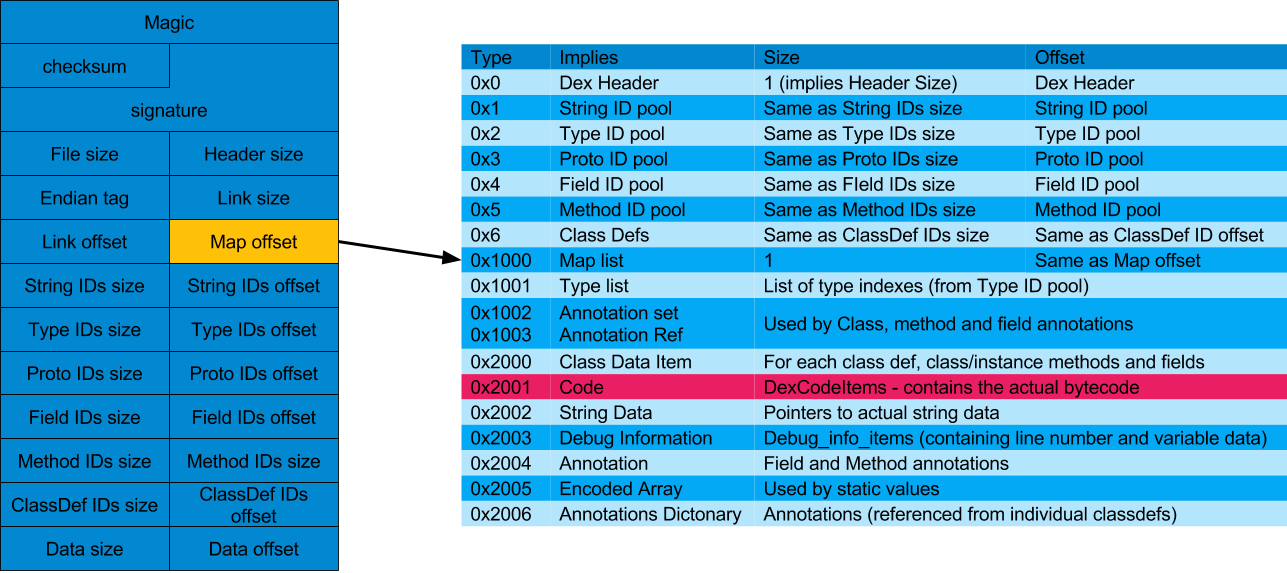
\includegraphics[width=0.8\textwidth]{data/dex.png}
    \caption{\gls{dex} file format \cite{andevconDalvikART}}
    \label{fig:dex}
\end{figure}
\newline
\newline
Dex bytecode supports optimization, improvements for the underlying architecture can be applied to the bytecode upon installation.
The resulting \gls{dex} file is called \gls{odex}.
The optimizations are executed by a program called dexopt which is part of the Android platform.
For the \gls{dvm} it makes no difference whether \gls{dex} or \gls{odex} files are executed, except speed improvements.
\newline
Like Java bytecode, \gls{dex} bytecode has a serious downside.
Since the bytecode is pretty simple to understand, decompilation is easily done.
At the same time, protection is rarely applied by the developers.
This makes these applications an easy target for reverse engineering.
